\raggedright
\section{PCA}
Principal Component Analysis (PCA) was performed on the selected numerical variables to reduce dimensionality and identify the main axes of variation within the customer data. The analysis focuses on understanding the underlying structure defined by customer demographics and purchasing behaviour.

The inertia (variance) explained by each principal component is visualized bellow.

\begin{figure}[H]
    \centering
    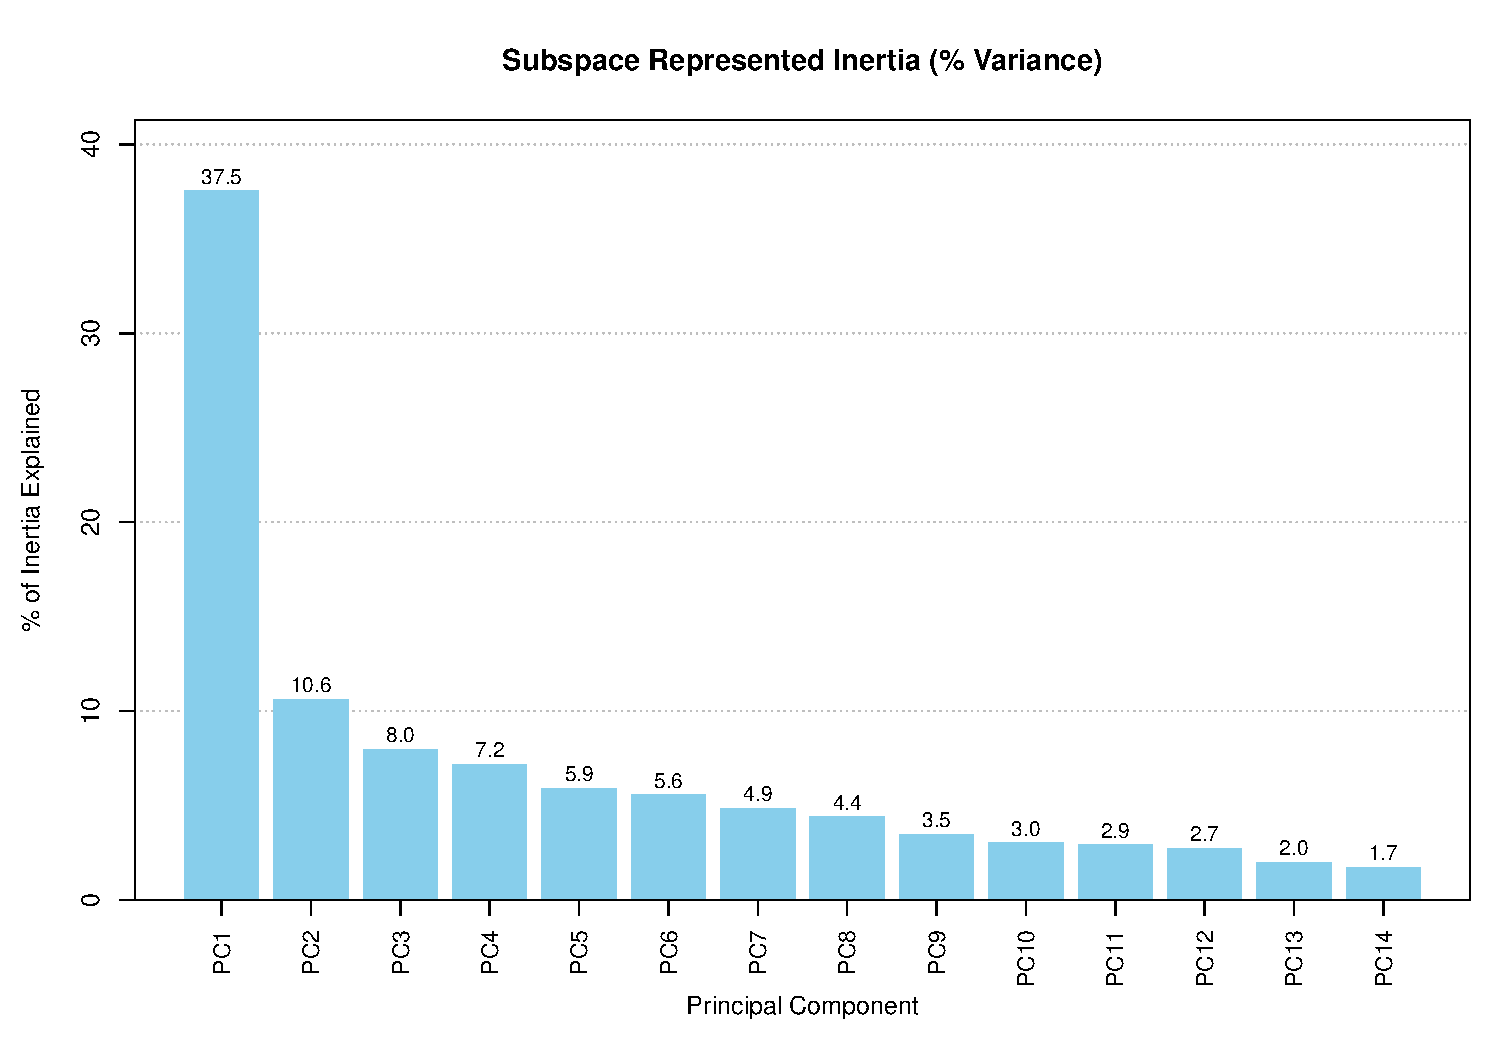
\includegraphics[width=0.8\linewidth]{Imatges/represented_inertia_plot.pdf}
    \caption{Scree plot showing eigenvalues (variance) of each principal component}
    \label{fig:scree_plot}
\end{figure}

\begin{figure}[H]
    \centering
    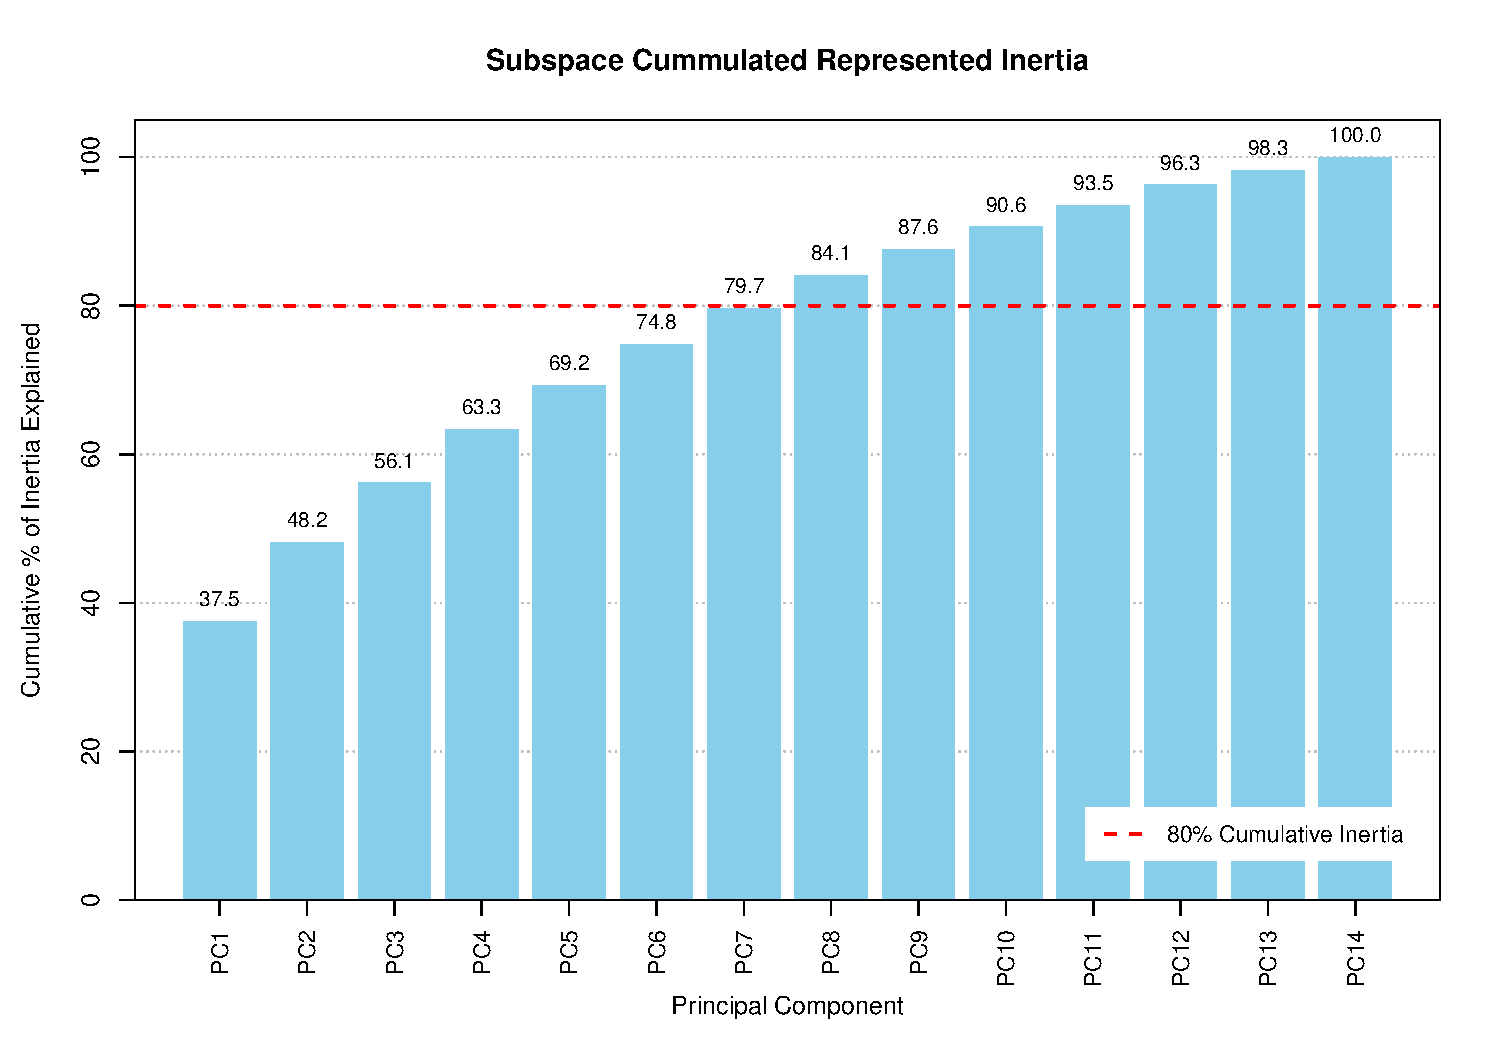
\includegraphics[width=0.8\linewidth]{Imatges/cummulated_inertia_plot.pdf}
    \caption{Cumulative explained variance by principal components}
    \label{fig:cumulative_variance}
\end{figure}

Figure \ref{fig:scree_plot} shows the percentage of variance explained by each component individually. PC1 clearly dominates, capturing 37.5\% of the variance.

Figure \ref{fig:cumulative_variance} shows the cumulative variance explained. Based on Kaiser's criterion (eigenvalues > 1, corresponding to components explaining more variance than an average original variable), to avoid excessive combinations, the first four principal components are selected for potential analysis. These four components cumulatively explain 63.3\% of the total variance and will help us determine which dimensions to focus on.



% Individual factor maps - individual figures
\begin{figure}[H]
    \centering
    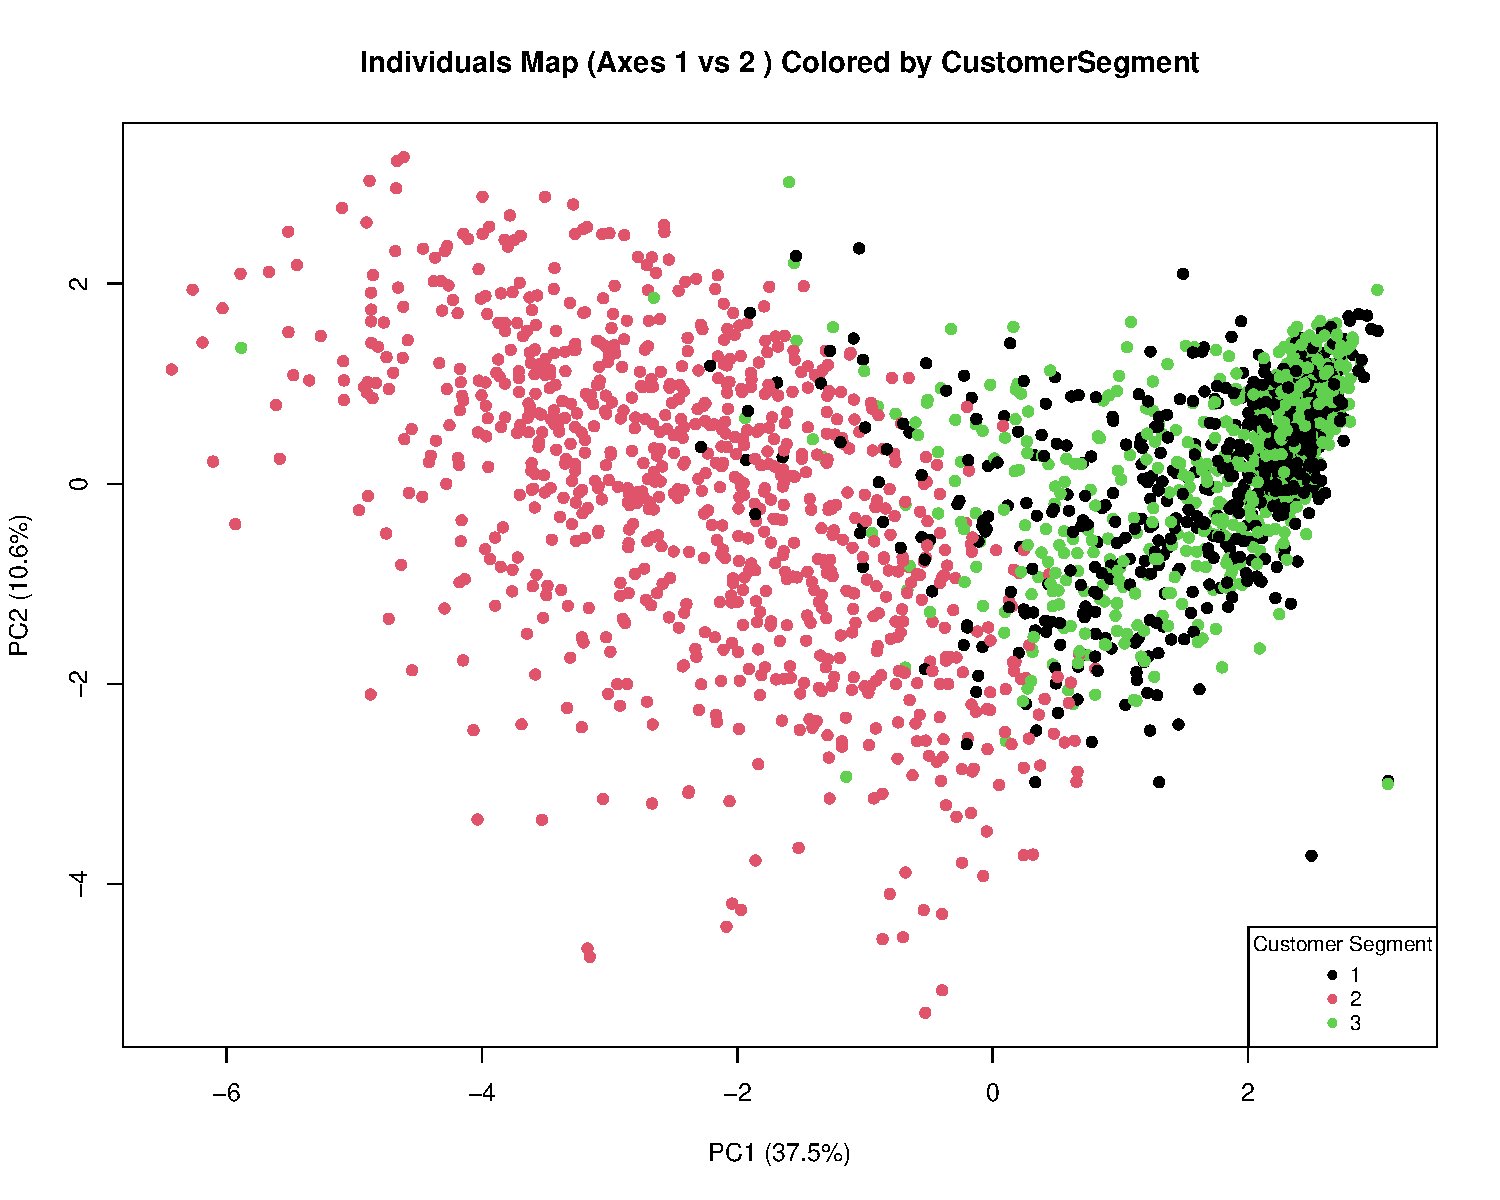
\includegraphics[width=0.8\linewidth]{Imatges/individuals_map_1_2.pdf}
    \caption{Individual factor map for dimensions 1 and 2}
    \label{fig:individuals_map_1_2}
\end{figure}

\begin{figure}[H]
    \centering
    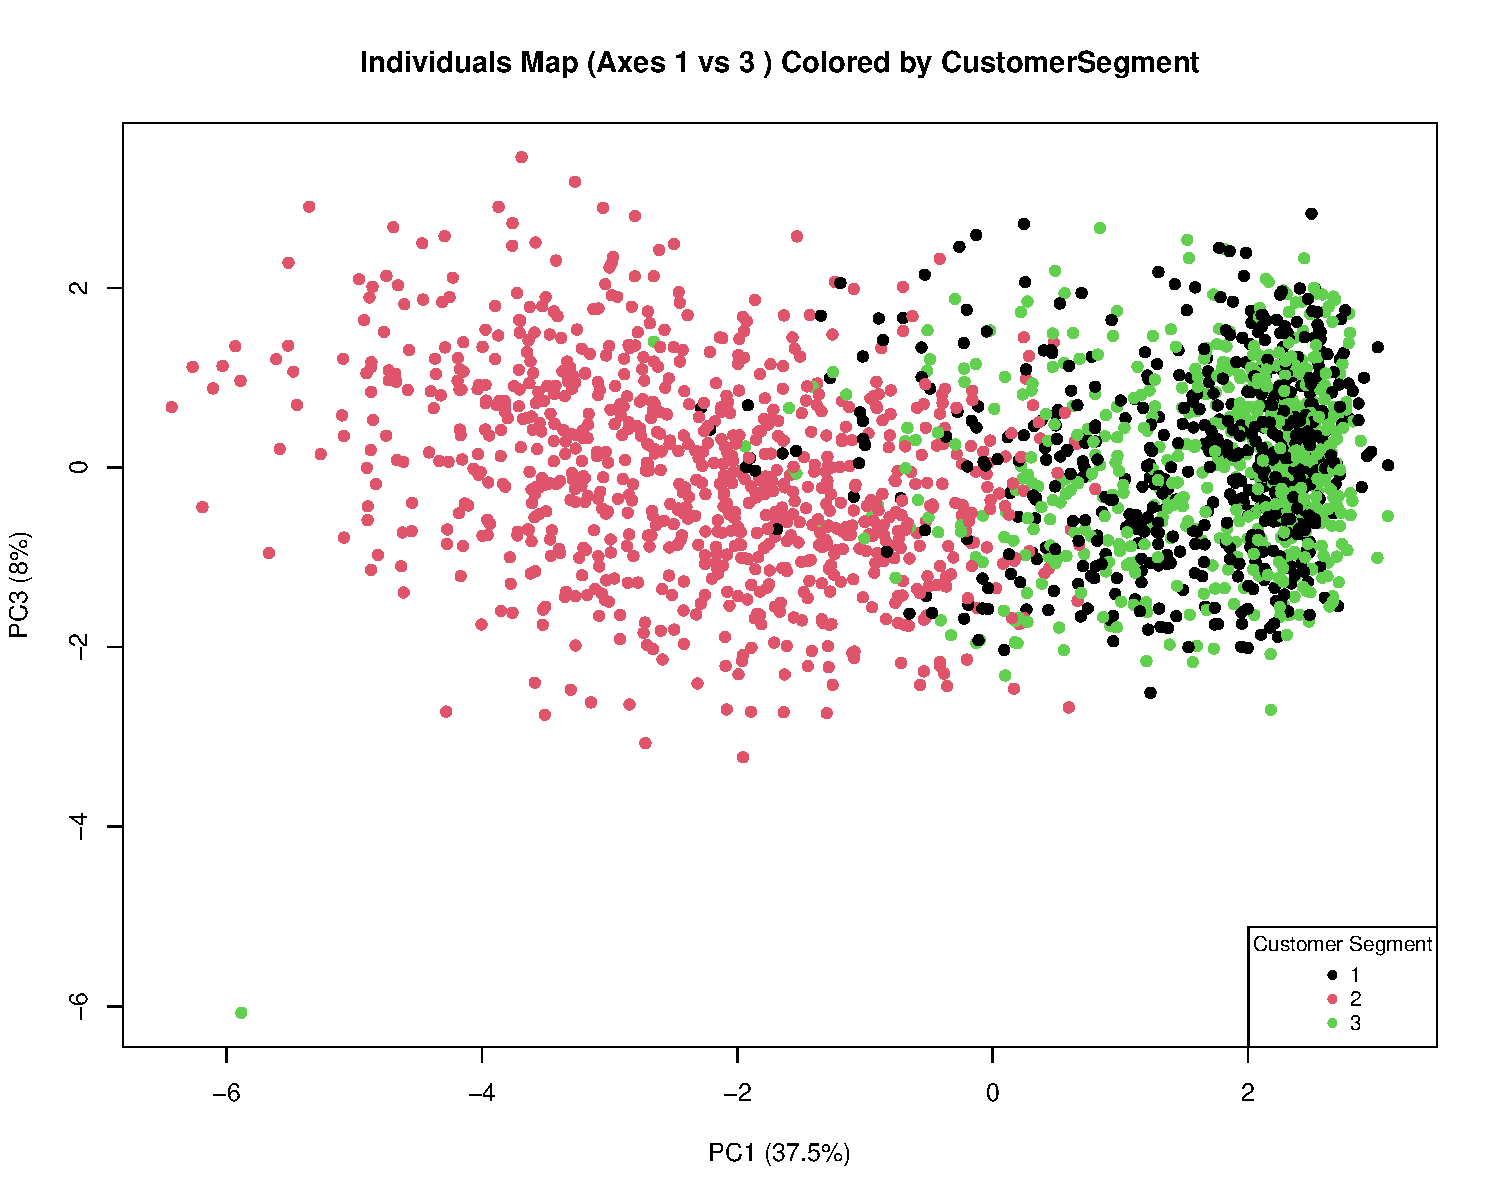
\includegraphics[width=0.8\linewidth]{Imatges/individuals_map_1_3.pdf}
    \caption{Individual factor map for dimensions 1 and 3}
    \label{fig:individuals_map_1_3}
\end{figure}

\begin{figure}[H]
    \centering
    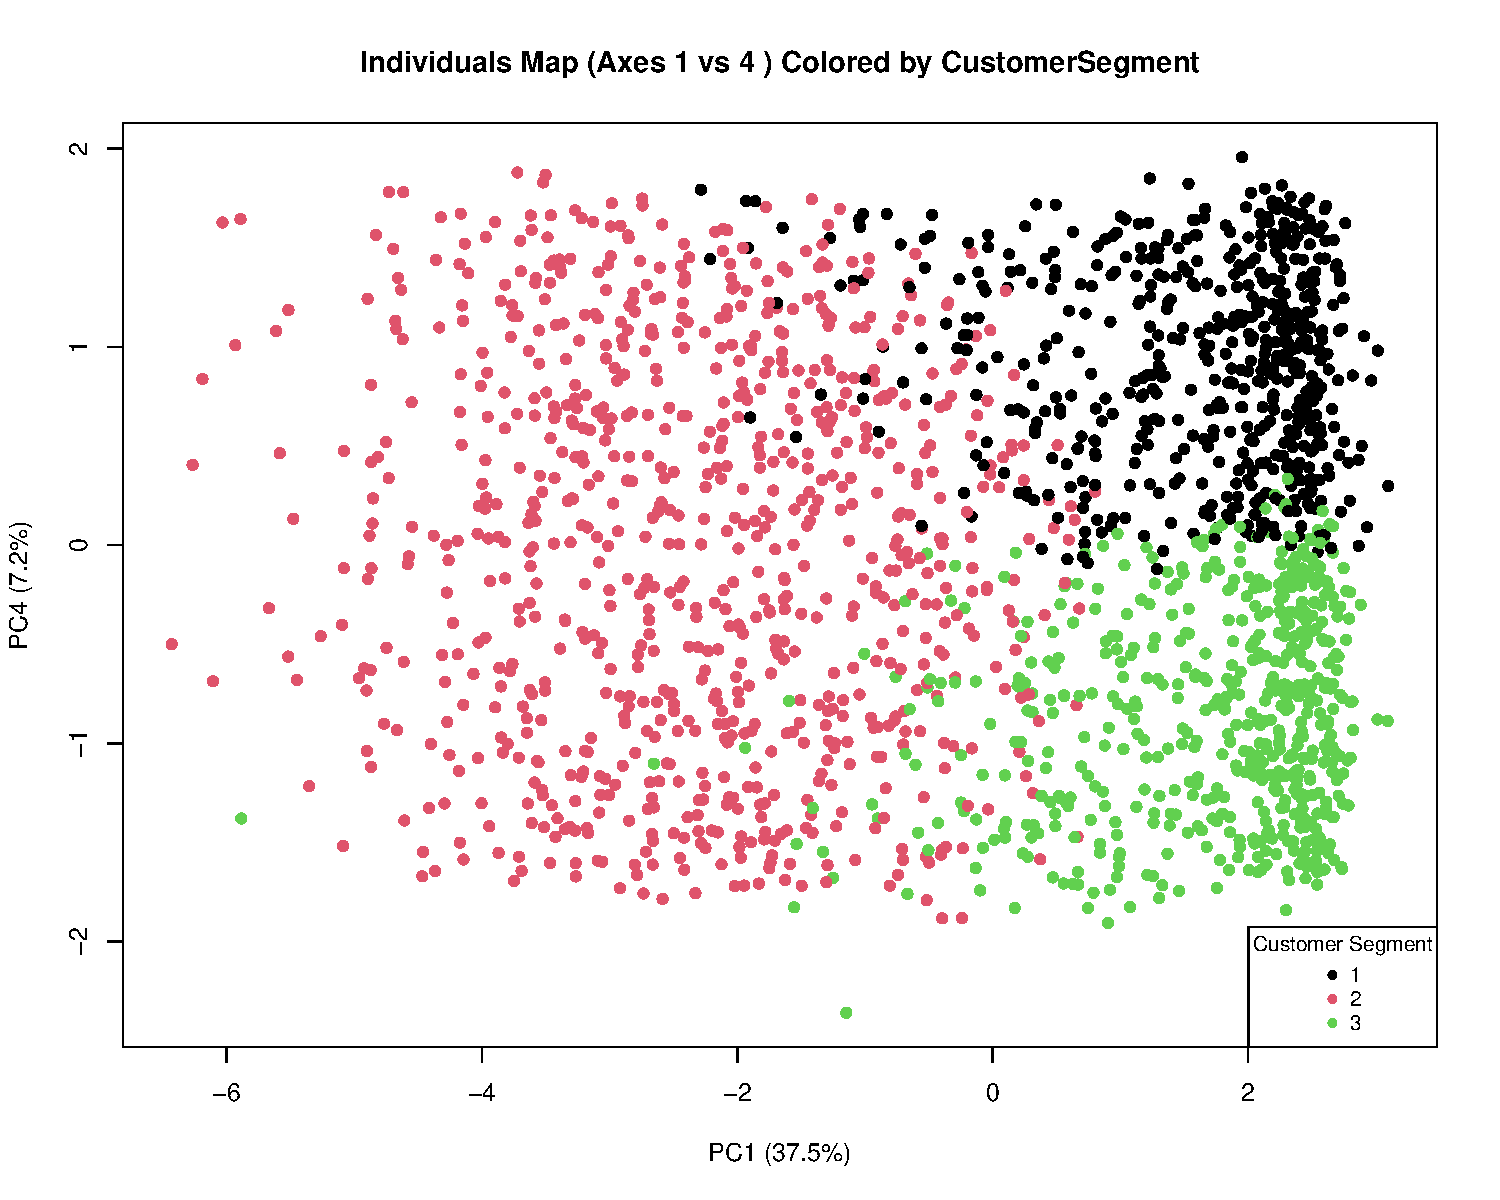
\includegraphics[width=0.8\linewidth]{Imatges/individuals_map_1_4.pdf}
    \caption{Individual factor map for dimensions 1 and 4}
    \label{fig:individuals_map_1_4}
\end{figure}

\begin{figure}[H]
    \centering
    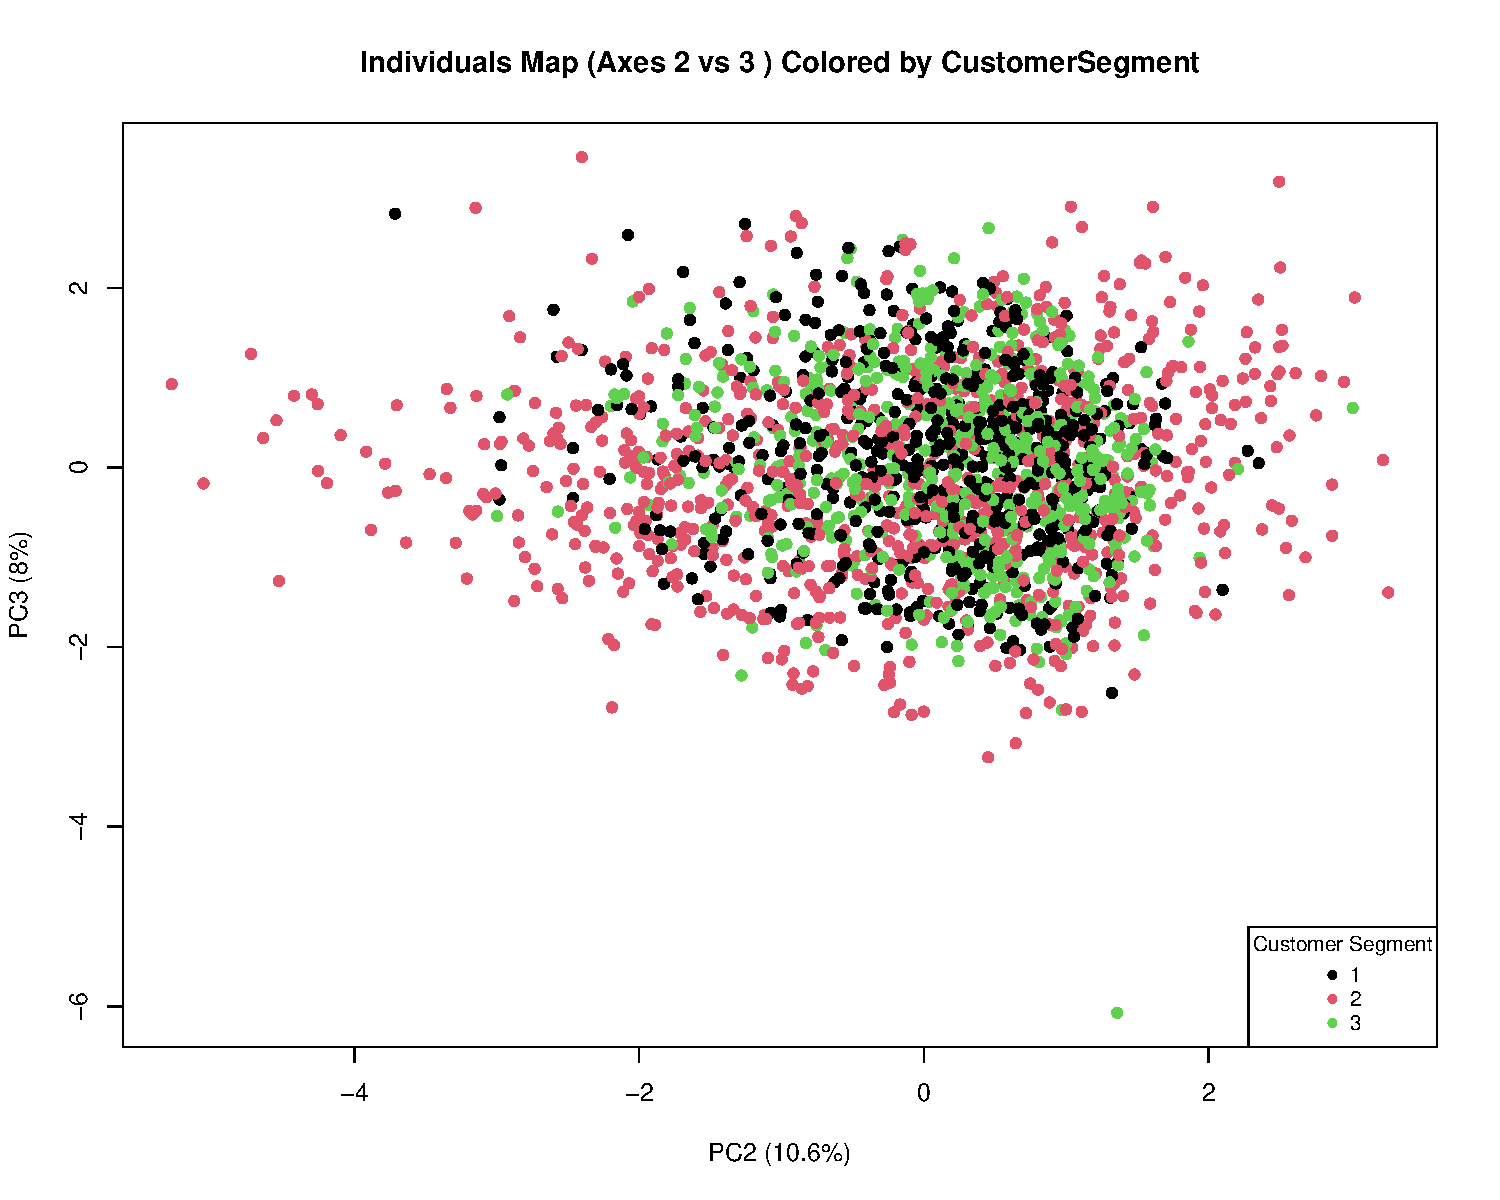
\includegraphics[width=0.8\linewidth]{Imatges/individuals_map_2_3.pdf}
    \caption{Individual factor map for dimensions 2 and 3}
    \label{fig:individuals_map_2_3}
\end{figure}

\begin{figure}[H]
    \centering
    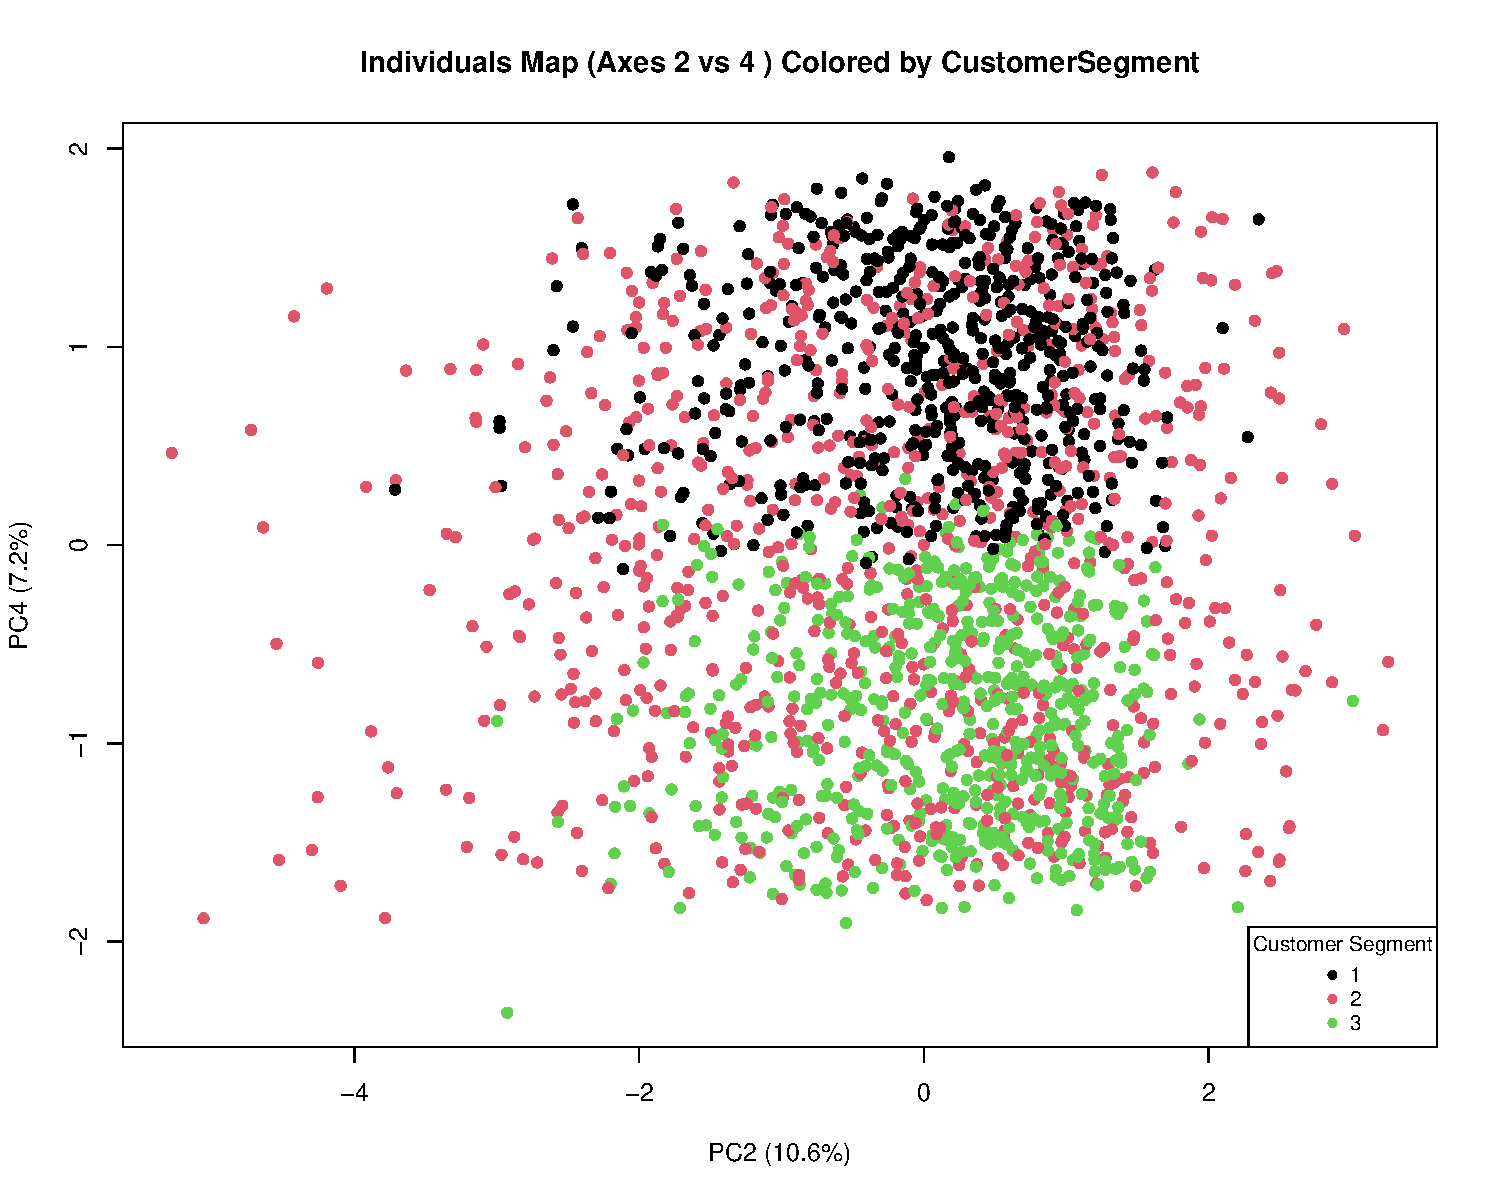
\includegraphics[width=0.8\linewidth]{Imatges/individuals_map_2_4.pdf}
    \caption{Individual factor map for dimensions 2 and 4}
    \label{fig:individuals_map_2_4}
\end{figure}

\begin{figure}[H]
    \centering
    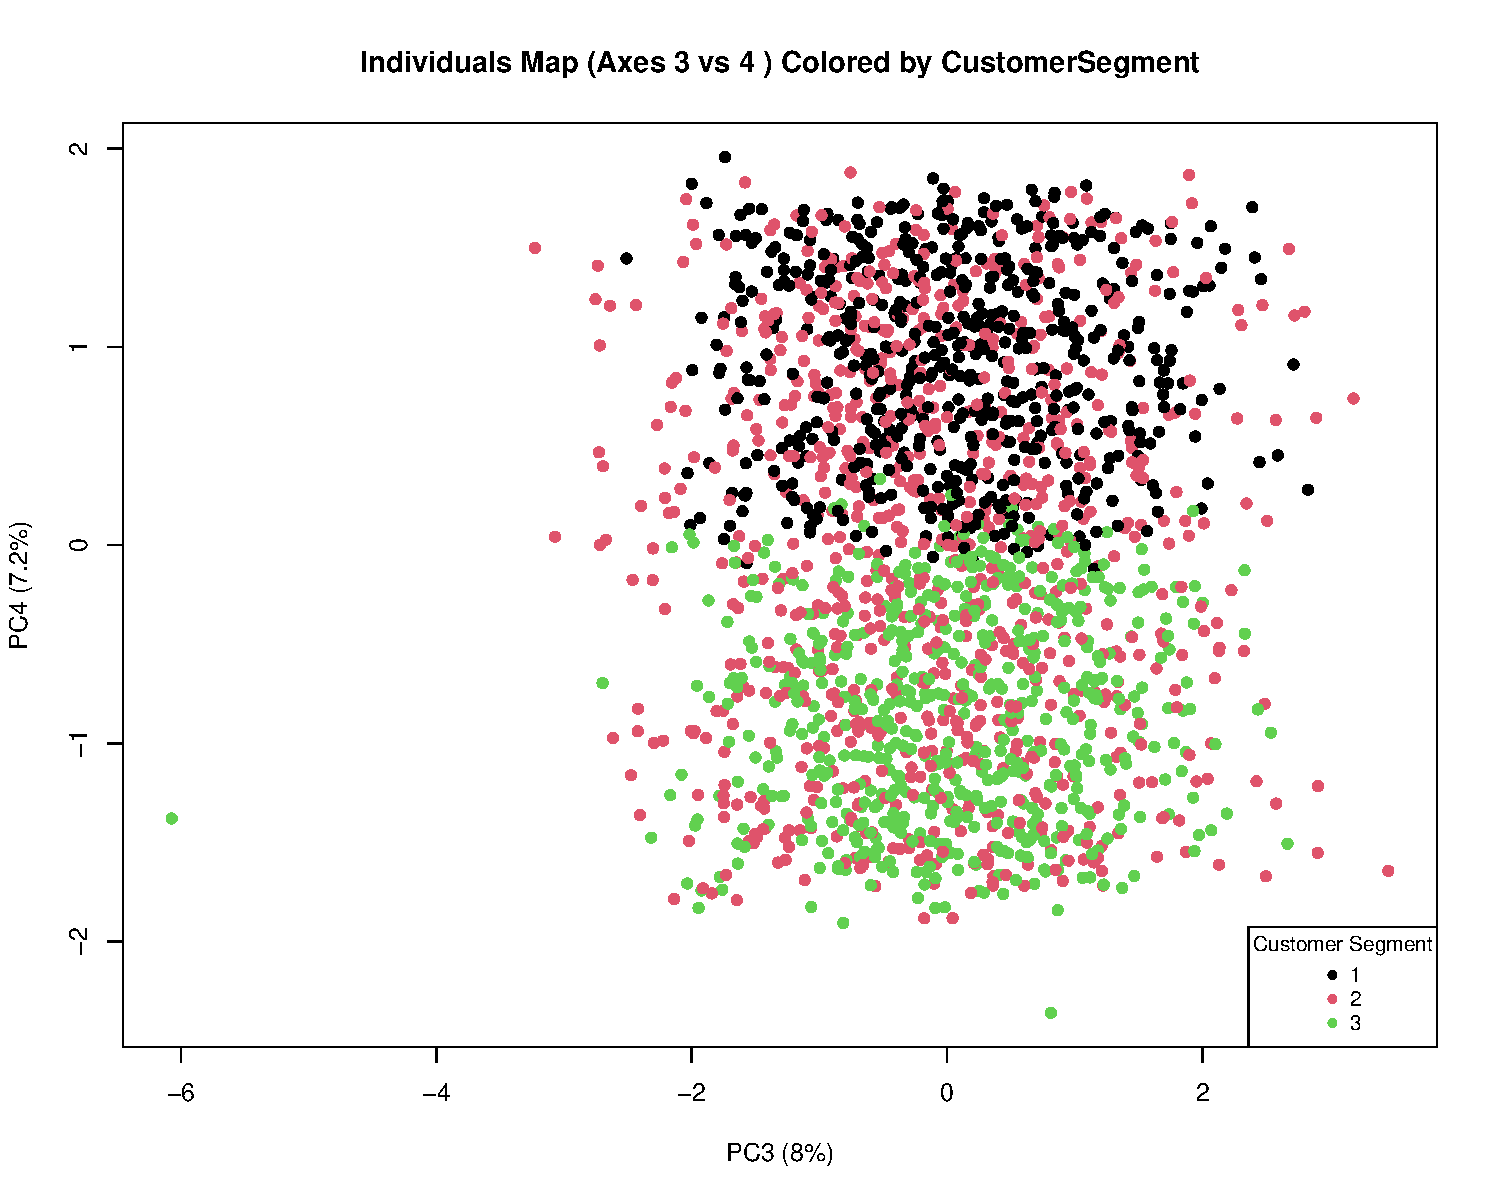
\includegraphics[width=0.8\linewidth]{Imatges/individuals_map_3_4.pdf}
    \caption{Individual factor map for dimensions 3 and 4}
    \label{fig:individuals_map_3_4}
\end{figure}

\newpage
Following an analysis of the results, PC1 vs PC2 plane was chosen for detailed interpretation as it captures the largest variance and shows the clearest separation. We will also focus on PC1 vs PC3 to offer a more in-depth analysis.




% Numerical - Qualitative variables maps PC1-PC2
\begin{figure}[H]
    \centering
    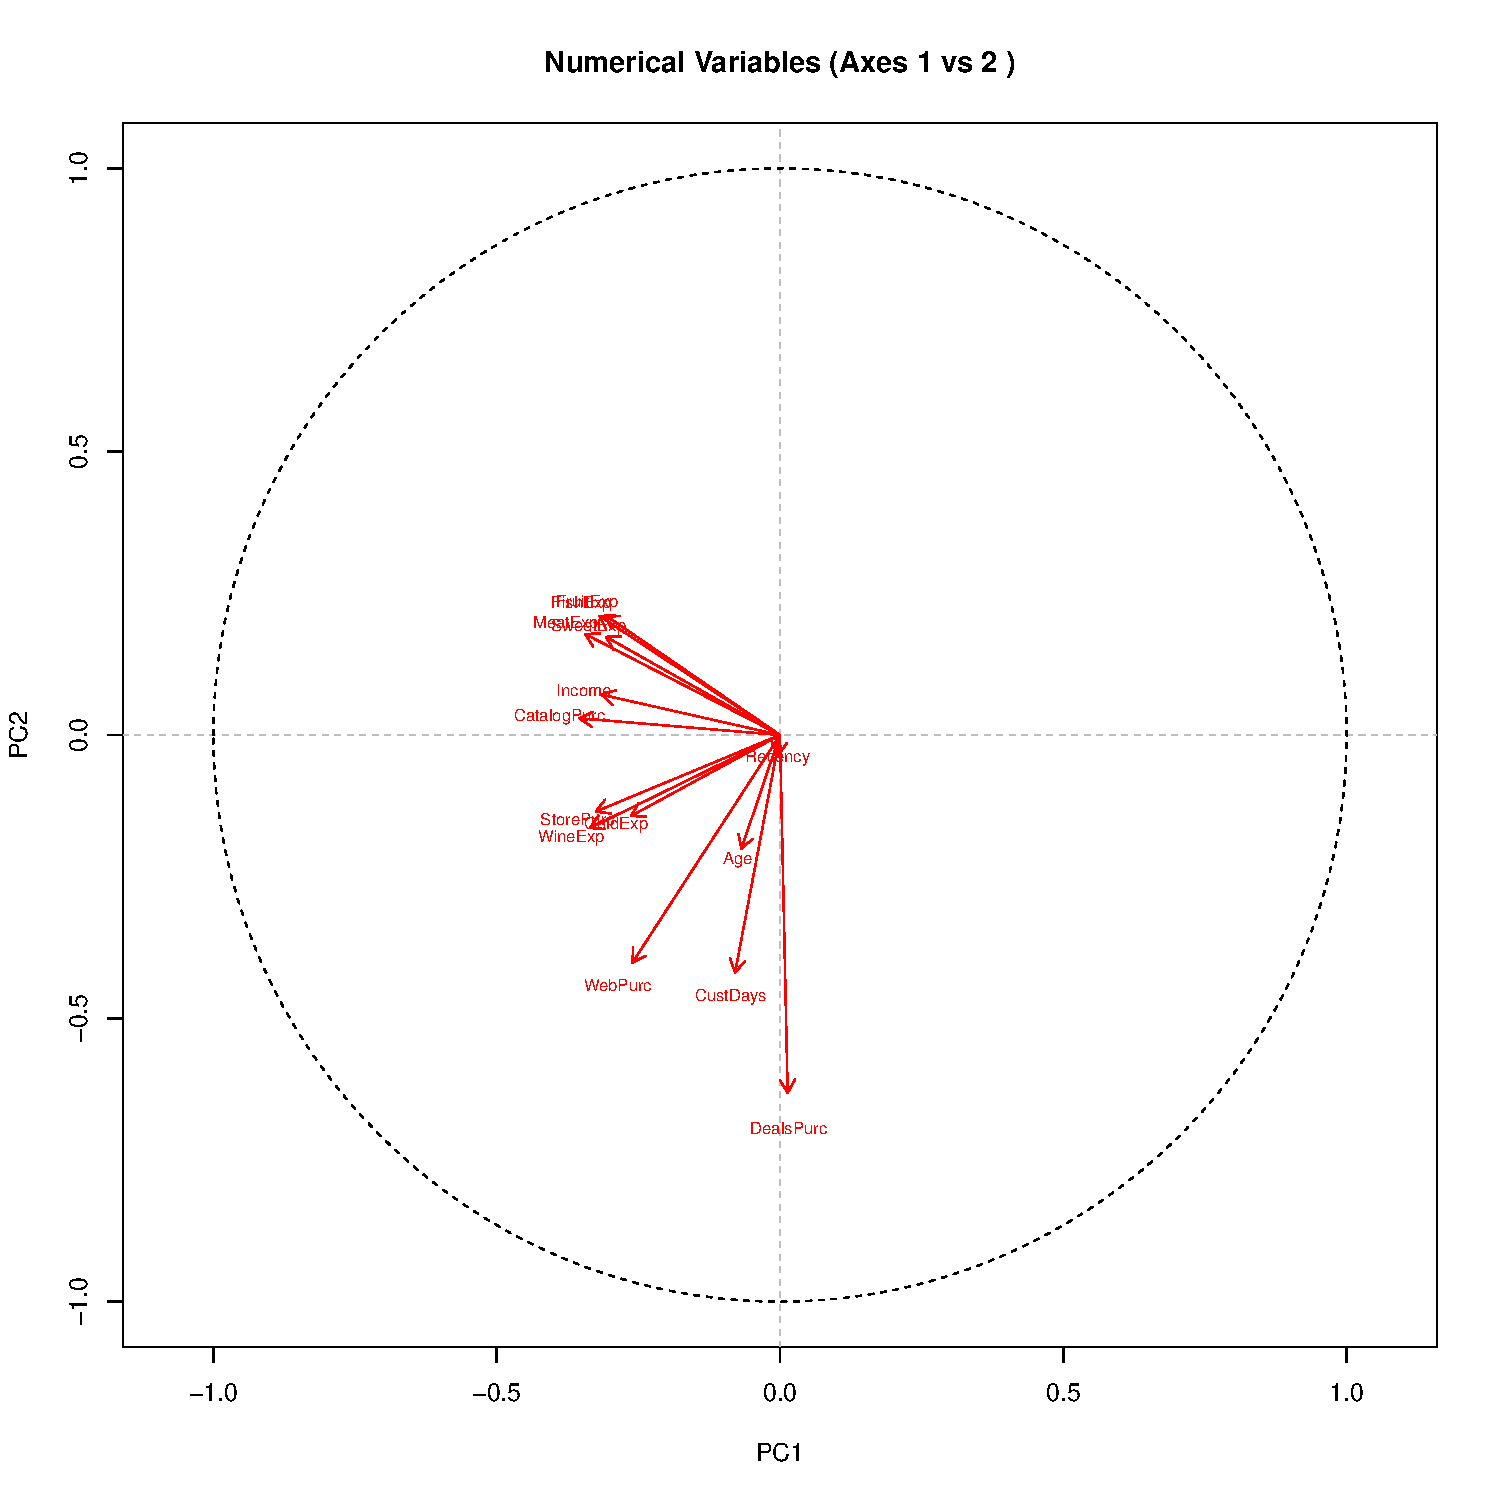
\includegraphics[width=0.9\linewidth]{Imatges/numerical_variables_map_1_2.pdf}
    \caption{Numerical variables correlation circle for dimensions 1 and 2}
    \label{fig:numerical_map_1_2}
\end{figure}

\begin{figure}[H]
    \centering
    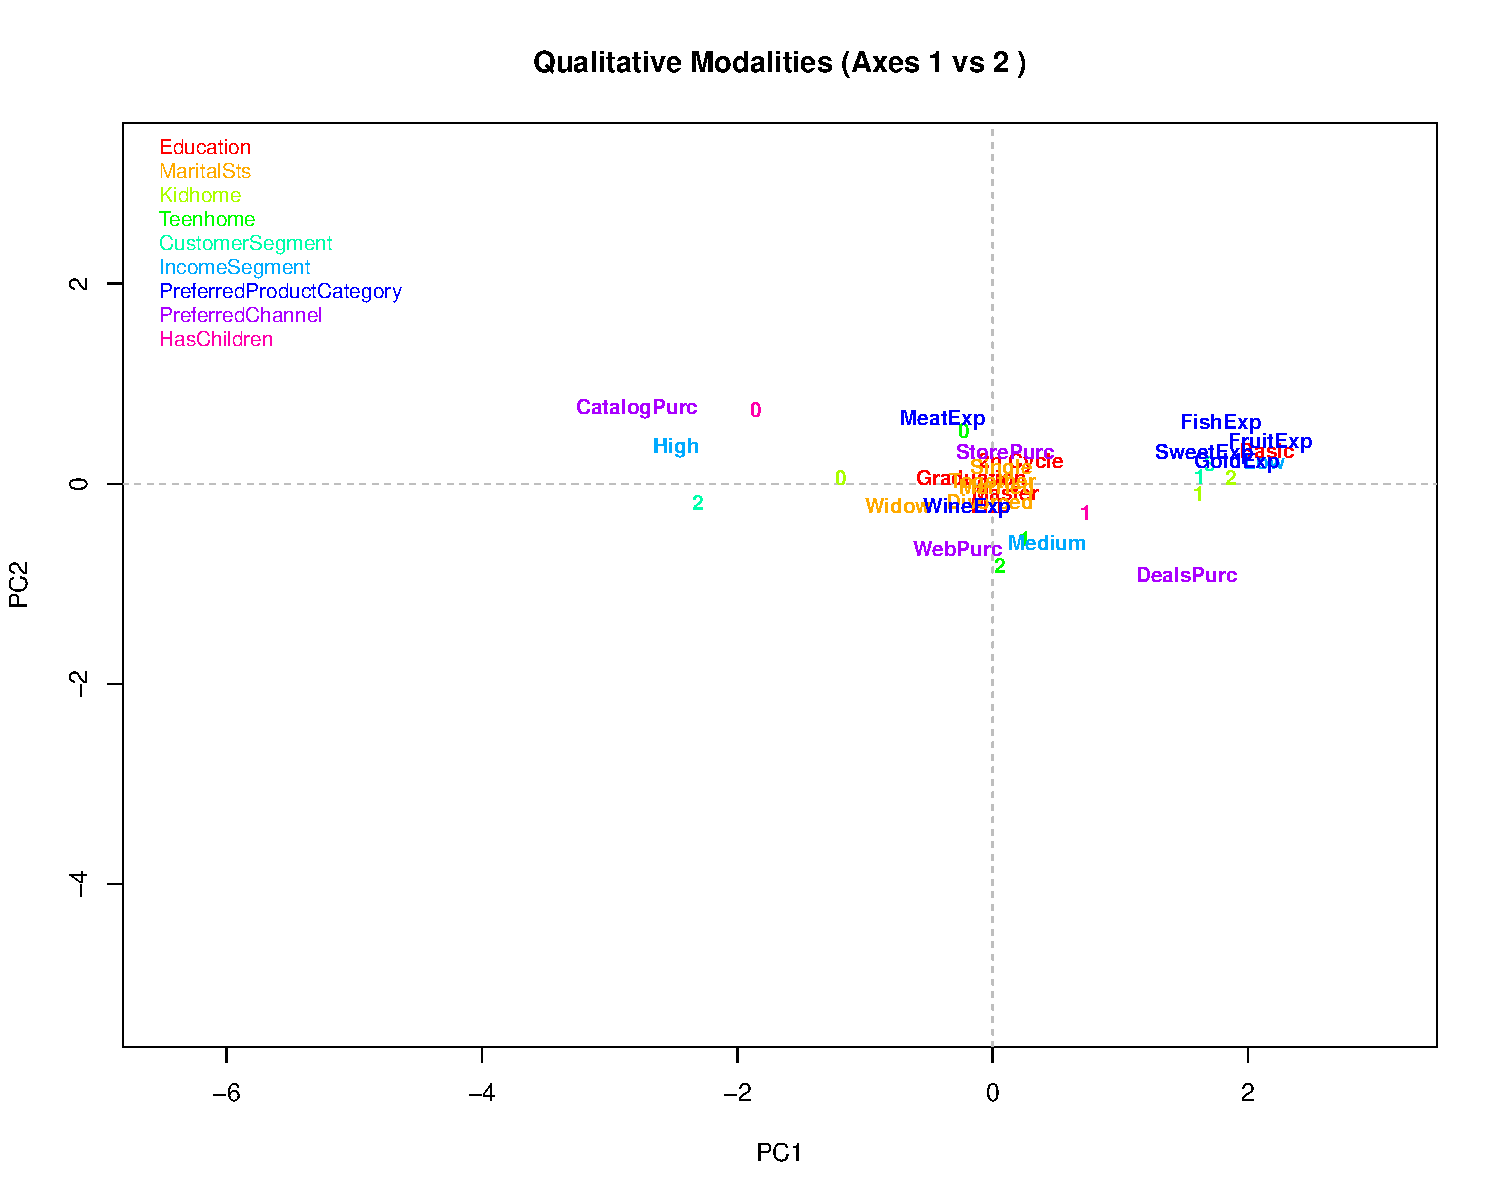
\includegraphics[width=0.9\linewidth]{Imatges/qualitative_modalities_map_1_2.pdf}
    \caption{Qualitative modalities map for dimensions 1 and 2}
    \label{fig:qualitative_map_1_2}
\end{figure}

Based on the variable projections, the first two principal components can be interpreted as follows:

\begin{itemize}
    \item \textbf{Axis 1 (PC1: 37.5\%): Customer Value.} The positive side (right) is strongly associated with higher \texttt{Income}, higher spending across most categories (especially \texttt{WineExp}, \texttt{MeatExp}, \texttt{CatalogPurc}), and \texttt{CustomerSegment 2}. The negative side (left) corresponds to lower income, lower spending, \texttt{CustomerSegment 1} \& \texttt{3}, and having younger children (\texttt{Kidhome 1}). This axis primarily differentiates customers based on their overall economic value and engagement.
    
    \item \textbf{Axis 2 (PC2: 10.6\%): Lifestage \& Channel Preference.} The positive side (top) is strongly characterized by \texttt{DealsPurc} and \texttt{WebPurc}, along with having teenagers at home (\texttt{Teenhome 1}, \texttt{Teenhome 2}). The negative side (bottom) is associated with having no children or teens (\texttt{HasChildren 0}, \texttt{Teenhome 0}) and potentially more traditional purchasing (\texttt{CatalogPurc}). This axis differentiates customers based on their life stage (presence of teens) and their preferred shopping channels and deal sensitivity.
\end{itemize}


% Numerical - Qualitative variables maps PC1-PC3
\begin{figure}[H]
    \centering
    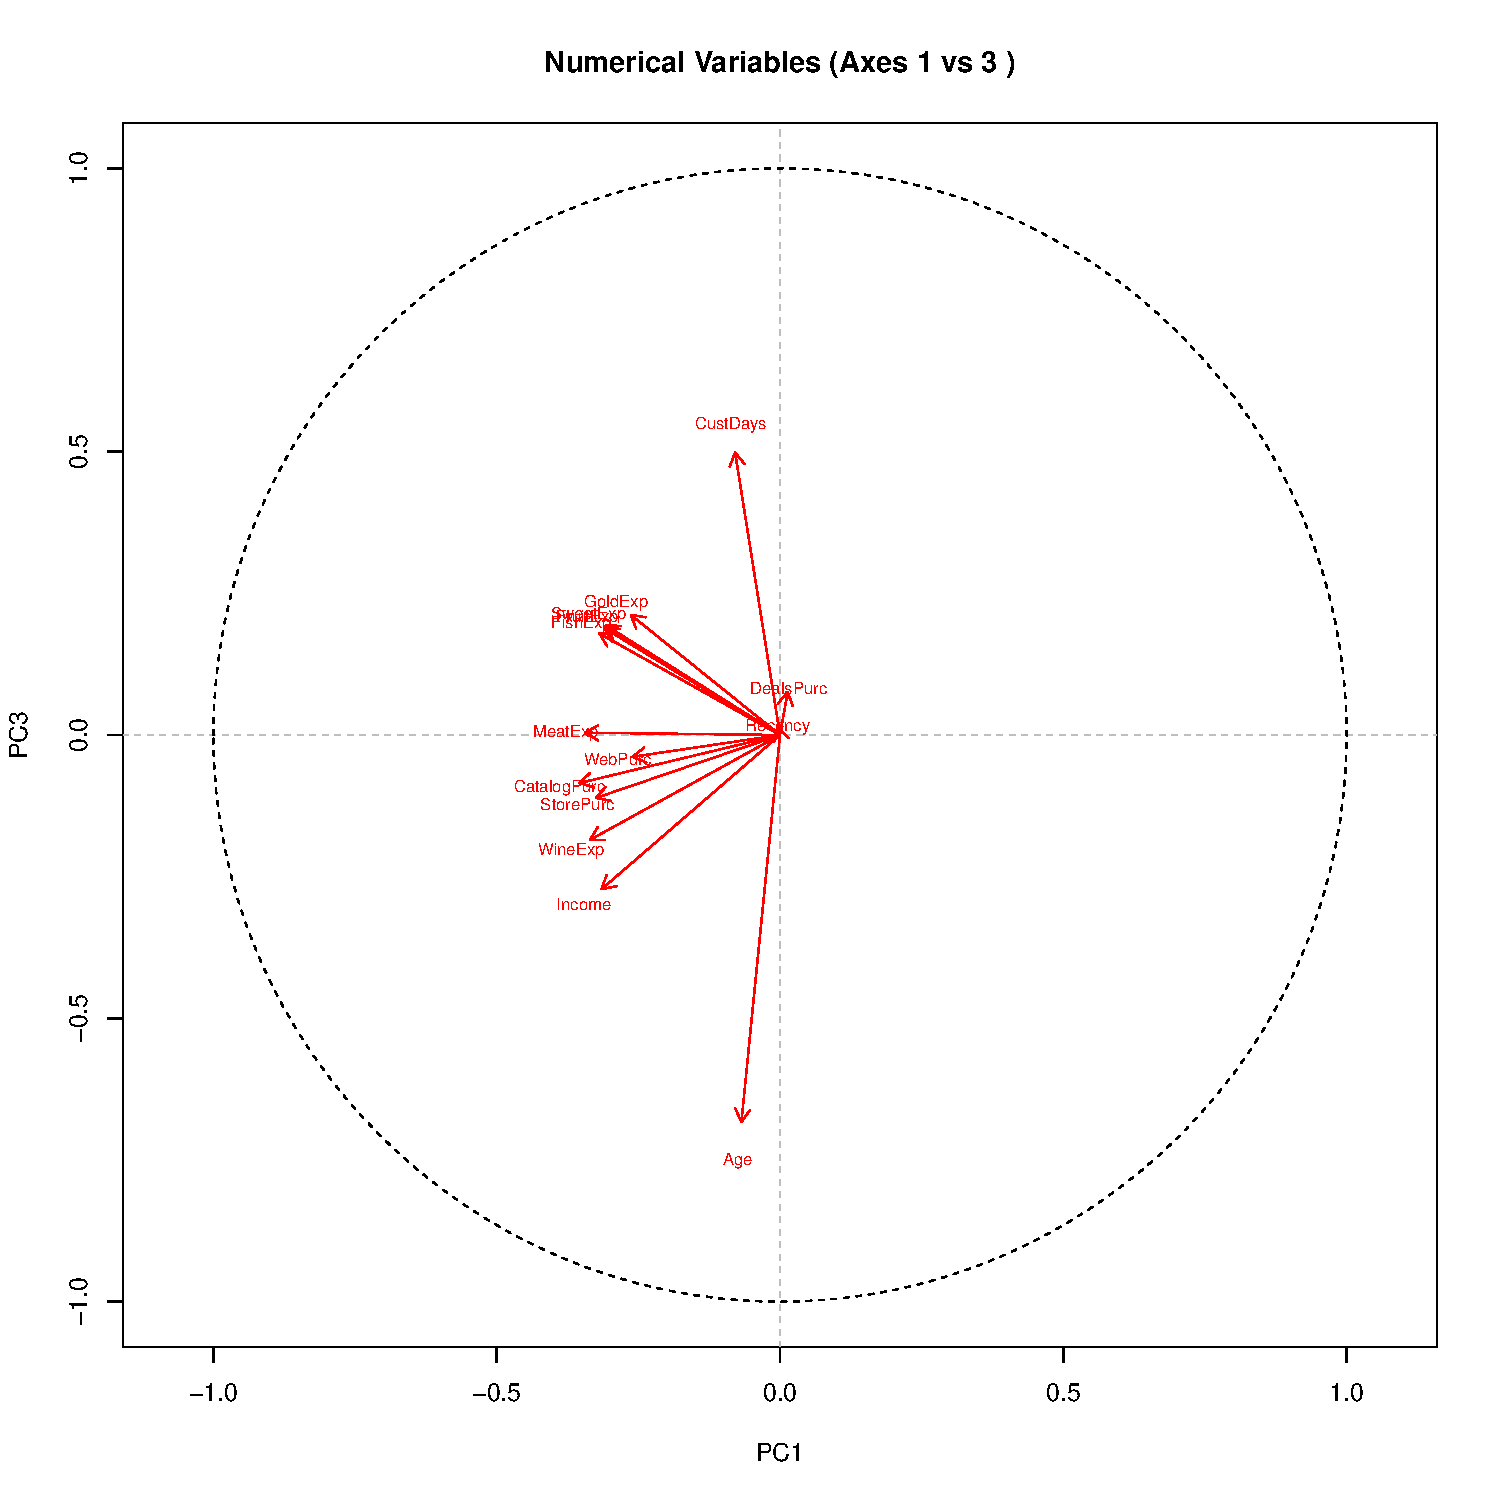
\includegraphics[width=0.9\linewidth]{Imatges/numerical_variables_map_1_3.pdf}
    \caption{Numerical variables correlation circle for dimensions 1 and 3}
    \label{fig:numerical_map_1_3}
\end{figure}

\begin{figure}[H]
    \centering
    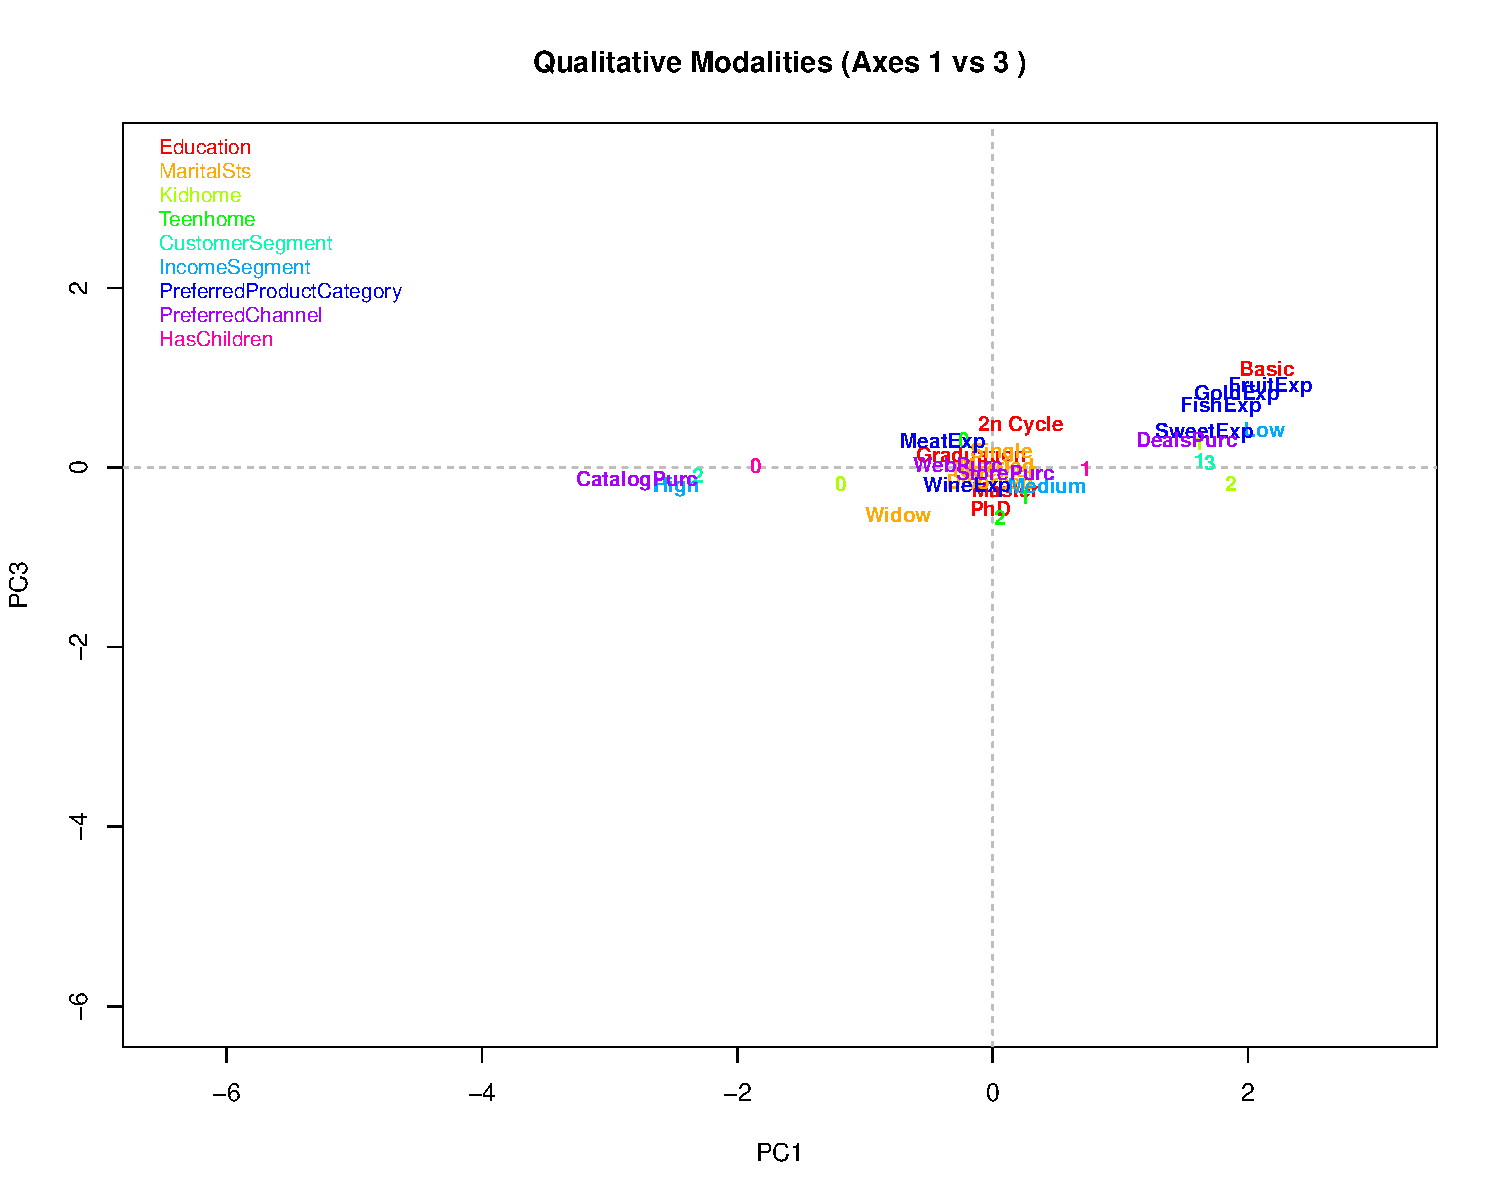
\includegraphics[width=0.9\linewidth]{Imatges/qualitative_modalities_map_1_3.pdf}
    \caption{Qualitative modalities map for dimensions 1 and 3}
    \label{fig:qualitative_map_1_3}
\end{figure}


Based on the variable projections, the first and third principal components can be interpreted as follows:

\begin{itemize}
    \item \textbf{Axis 1 (PC1: 37.5\%): Customer Value.} \textit{(Interpretation remains the same)} The positive side (right) is strongly associated with higher \texttt{Income}, higher spending across most categories (especially \texttt{WineExp}, \texttt{MeatExp}, \texttt{CatalogPurc}), and \texttt{CustomerSegment 2}. The negative side (left) corresponds to lower income, lower spending, \texttt{CustomerSegment 1} \& \texttt{3}, and having younger children (\texttt{Kidhome 1}). This axis primarily differentiates customers based on their overall economic value and engagement.
    
    \item \textbf{Axis 3 (PC3: 8.0\%): Customer Maturity \& Tenure.} The positive side (top) is strongly characterized by higher \texttt{Age}. The negative side (bottom) is associated with longer customer tenure (\texttt{CustDays}). This axis appears to differentiate customers based on their age and how long they have been a customer, potentially contrasting older, perhaps newer high-value customers from younger, more established ones.
\end{itemize}
